\documentclass{article}
\usepackage[utf8]{inputenc}
\usepackage{geometry}
 \geometry{
 a4paper,
 total={170mm,257mm},
 left=20mm,
 top=20mm,
 }
 \usepackage{graphicx}
 \usepackage{titling}
 \usepackage{amssymb}
 \usepackage{natbib}

\title{Testing the Effectiveness, Convergence, and Stability\\of Search-Based Hyperparameter Optimizers }
\author{
    Fernando Berti Cruz Nogueira (abert036@uottawa.ca), 
    Kelvin Mock (kmock073@uOttawa.ca)
}
 
\usepackage{fancyhdr}
\setlength{\headheight}{12.5pt}
\addtolength{\topmargin}{-0.5pt}
\fancypagestyle{plain}{%  the preset of fancyhdr 
    \fancyhf{} % clear all header and footer fields
    \fancyhead[L]{CSI 5186 - AI-enabled Software Verification and Testing, Final Report (Fall 2025)}
}
\makeatletter
\def\@maketitle{%
  \newpage
  \null
  \vskip 1em%
  \begin{center}%
  \let \footnote \thanks
    {\LARGE \@title \par}%
    \vskip 1em%
    %{\large \@date}%
  \end{center}%
  \par
  \vskip 1em}
\makeatother

\usepackage{float}
\usepackage{amsmath}
\usepackage{xcolor}
\usepackage{array}
\usepackage{booktabs}
\usepackage{multirow}
\usepackage{tabularx}
\usepackage{tikz}
\usetikzlibrary{positioning}
\usepackage[colorlinks=true,citecolor=blue,linkcolor=blue]{hyperref}
\begin{document}
\maketitle

\noindent\begin{tabular}{@{}ll}
    Students & \theauthor\\
    Lecturer & Dr. Shiva Nejati (snejati@uottawa.ca)
\end{tabular}

\begin{abstract}
Hyperparameter optimization is a critical but computationally expensive task for developing effective machine learning models. This report presents an empirical study comparing a Randomized Search (RS) baseline against two representative metaheuristics: a Genetic Algorithm (GA) and Particle Swarm Optimization (PSO). This selection is made to contrast two primary search strategies: global exploration (GA) and local exploitation (PSO). We evaluate the ability of these algorithms to optimize the hyperparameters of three distinct machine learning models (Decision Tree, k-Nearest Neighbors, and a Convolutional Neural Network) on the grayscale CIFAR-10 dataset~\cite{krizhevsky2009learning}. To ensure a fair and balanced assessment we define a composite fitness function. We evaluate the optimizers across three quality attributes: effectiveness (solution quality), convergence (improvement over a fixed evaluation budget), and stability (consistency across runs). The empirical results will be validated using statistical tests to provide statistically grounded conclusions.
\end{abstract}

\section{Introduction}

The performance of machine learning models often depends on their hyperparameters' high-level configuration variables like learning rate or batch size that control the training process. Finding the optimal set of these configurations, or Hyperparameter Optimization (HPO), is a significant and resource-intensive bottleneck in model development.

HPO can be framed as a software verification problem. In this context, the model is the software under test and a "defect" being a suboptimal hyperparameter configuration that causes the model to fail its performance specifications, such as by exhibiting high loss, poor generalization or unstable training. HPO thus functions as a automated test drivers, searching the configuration space to find a set of hyperparameters that verifies the model's performance against a pre-defined quality specification.

\subsection{Evaluation Criteria}

We evaluate the optimizers across three quality attributes, as defined in the project proposal:

\begin{itemize}
    \item \textbf{Effectiveness}: The quality of the final solution found (i.e., the best fitness score achieved).
    \item \textbf{Efficiency}: The computational cost required to find a solution, measured in both fitness evaluations and wall-clock time.
    \item \textbf{Stability (Consistency)}: The consistency and reliability of the algorithm's performance across multiple independent runs.
\end{itemize}

\subsection{Research Questions}

This report seeks to answer the following research questions from the project proposal:

\begin{itemize}
    \item \textbf{RQ1}: How do representative metaheuristic algorithms compare against a randomized search baseline in terms of effectiveness and efficiency when performing HPO prior to training?
    \item \textbf{RQ2}: What is the difference in performance stability between the selected metaheuristic algorithms and traditional solutions like the randomized search baseline?
\end{itemize}


\section{Problem Formulation}

\subsection{Objective Function}

HPO is a black-box optimization problem. The objective function $f(\theta)$, which represents the model's performance for a given hyperparameter configuration $\theta$, presents many challenges: it is computationally expensive to evaluate, it is non-differentiable, and the search space $\Theta$ is often complex and of mixed-types (continuous, discrete, and categorical). These properties make HPO suitable for search-based metaheuristic techniques.

\subsection{Algorithm Selection}

\subsubsection{Baseline: Randomized Search}

RS is the standard scientific baseline for HPO. \citet{bergstra2012random} demonstrated empirically that RS is more efficient than Grid Search for HPO, as it does not waste evaluations on unimportant parameters. Therefore, any intelligent algorithm must demonstrate superiority over RS to be considered effective.

\subsubsection{Genetic Algorithm}

TODO

\subsubsection{Particle Swarm Optimization}

PSO models a swarm where individuals are strongly influenced by the single best-found solution. This behaviour leads to rapid convergence, often finding a "good-enough" solution quickly. This same strength can also be a weakness, as it may converge prematurely to a suboptimal solution. The swarm can rapidly cluster around the first local optimum it finds, losing diversity and becoming "stuck" before the true global optimum is found.

\section{Experiment}

\subsection{Models and Dataset}

\subsubsection{Dataset}

The CIFAR-10 dataset~\cite{krizhevsky2009learning} is a dataset for object recognition. It consists of \( 32 \times 32 \) colored images. There are 60000 images in total. Those images are in 10 balanced classes (so we do not need to worry about class imbalance issues). 

\paragraph{Preprocessing} We use a grayscale version of CIFAR-10. Those RGB images ($32 \times 32$ pixels) are converted to grayscale using $Y = 0.2125R + 0.7154G + 0.0721B$ and normalized to $[0, 1]$.

\subsubsection{Data Split}

\begin{itemize}
    \item Training Set: 45,000 images
    \item Validation Set: 5,000 images (for HPO fitness evaluation).
    \item Test Set: 10,000 images (held out for final model evaluation after HPO is complete).
\end{itemize} 

\subsubsection{Models}

In our study, we aim to cover the following machine learning models:

\paragraph{Decision Tree (DT)} DT is the simplest model in nature. It is tree-based which suggests making predictions based on binary predicates. Its architecture is not complex for training and it is also highly explainable to non-technical persons. It is also widely used in real-world production-grade systems like autonomous vehicles \cite{autonomous-vehicle-appl}. Given its simplicity and popularity, we start our analysis on exploring what parameters minimally have to be tuned for the simplest model, and how it performs during tuning with metaheuristics. For simplicity, a prebuilt structure from \cite{dt-scikit} is used.

\paragraph{K-Nearest Neighbors (KNN)} KNN is another simple model which predicts based on the class of a nearest neighbor among existing data instances. From the perspective of explainability, a prior work \cite{mygithub-drugconsumpML} suggests that, depending on datasets, sometimes a KNN classifier could be linear-based, but in the case of an image dataset, KNN in our experiment are predicting from highly dimensional image arrays, whose predictions need to be generalized by a kernel-based explainer. The model's architecture itself is not complex but the dataset involved could be a bit heavier training task. We used it as another type of model in our experiment. For simplicity, a prebuilt structure from \cite{knn-scikit} is used.

\paragraph{Convolutional Neural Network (CNN)} While the above models might exhibit a simpler architecture, CNN, on the other hand, is a common deep learning architecture in practical works, which helps learning image recognition tasks more efficiently. It is a fully-connected neural network architecture which leverages operations known as "convolutions". Each of which utilizes a subset of pixels, known as a "kernel", or a "filter", iteratively learn those patterns. Custom neural networks generally, in the real-world, involve far more hyper-parameters during their training, and thus, tuning them is computationally much heavier than those prebuilt surrogate models. However, bad hyper-parameters could also increase the resulting error rate of the model \cite{metaheuristics-cookbook}. Therefore, a suitable metaheuristic search here comes with an important role to help determine the best set of hyper-parameters with fewer resources than an exhaustive search. Figure~\ref{fig:cnn_arch} summarizes the CNN backbone used in our experiments.

\begin{figure}[ht]
\centering
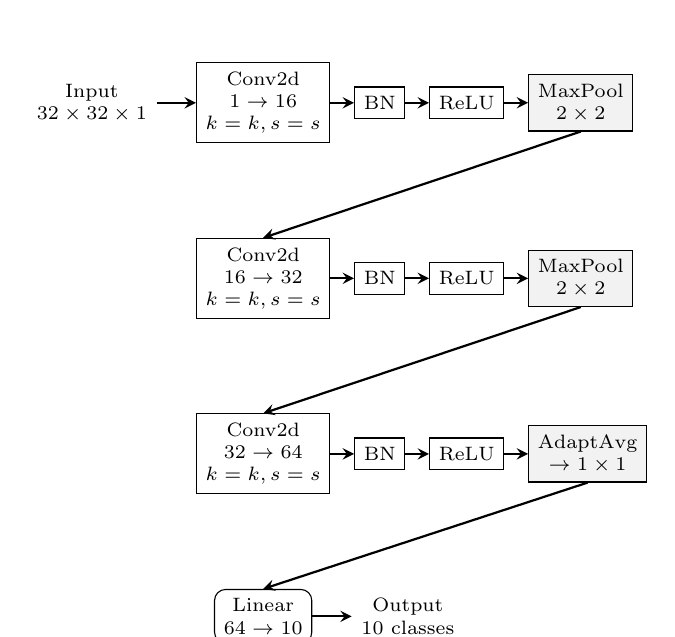
\begin{tikzpicture}[
    node distance=0.6cm,
    conv/.style={draw=black, align=center, font=\scriptsize},
    norm/.style={draw=black, align=center, font=\scriptsize},
    act/.style={draw=black, align=center, font=\scriptsize},
    pool/.style={draw=black, align=center, fill=gray!10, font=\scriptsize},
    linear/.style={draw=black, align=center, rounded corners, font=\scriptsize},
    arrow/.style={->, thick, >=stealth},
]
    % Block 1
    \node[conv] (conv1) {Conv2d\\$1 \to 16$\\$k=k, s=s$};
    \node[norm, right=0.3cm of conv1] (bn1) {BN};
    \node[act, right=0.3cm of bn1] (relu1) {ReLU};
    \node[pool, right=0.3cm of relu1] (pool1) {MaxPool\\$2 \times 2$};
    
    % Block 2
    \node[conv, below=1.2cm of conv1] (conv2) {Conv2d\\$16 \to 32$\\$k=k, s=s$};
    \node[norm, right=0.3cm of conv2] (bn2) {BN};
    \node[act, right=0.3cm of bn2] (relu2) {ReLU};
    \node[pool, right=0.3cm of relu2] (pool2) {MaxPool\\$2 \times 2$};
    
    % Block 3
    \node[conv, below=1.2cm of conv2] (conv3) {Conv2d\\$32 \to 64$\\$k=k, s=s$};
    \node[norm, right=0.3cm of conv3] (bn3) {BN};
    \node[act, right=0.3cm of bn3] (relu3) {ReLU};
    \node[pool, right=0.3cm of relu3] (pool3) {AdaptAvg\\$\to 1 \times 1$};
    
    % Classifier
    \node[linear, below=1.2cm of conv3] (fc) {Linear\\$64 \to 10$};
    
    % Connections
    \draw[arrow] (conv1) -- (bn1);
    \draw[arrow] (bn1) -- (relu1);
    \draw[arrow] (relu1) -- (pool1);
    
    \draw[arrow] (conv2) -- (bn2);
    \draw[arrow] (bn2) -- (relu2);
    \draw[arrow] (relu2) -- (pool2);
    
    \draw[arrow] (conv3) -- (bn3);
    \draw[arrow] (bn3) -- (relu3);
    \draw[arrow] (relu3) -- (pool3);
    
    % Inter-block connections
    \draw[arrow] (pool1.south) -- (conv2.north);
    \draw[arrow] (pool2.south) -- (conv3.north);
    \draw[arrow] (pool3.south) -- (fc.north);
    
    % Input/Output
    \node[left=0.5cm of conv1, align=center, font=\scriptsize] (input) {Input\\$32 \times 32 \times 1$};
    \draw[arrow] (input) -- (conv1);
    
    \node[right=0.5cm of fc, align=center, font=\scriptsize] (output) {Output\\10 classes};
    \draw[arrow] (fc) -- (output);
\end{tikzpicture}
\caption{CNN Architecture. Note: $k$ (kernel size) and $s$ (stride) are optimized hyperparameters.}
\label{fig:cnn_arch}
\end{figure}

\paragraph{Significance of CNN} From several existing works, an HPO problem for CNN models specifically is consistently treated as a combinatorial optimization problem, and metaheuristics are used to efficiently navigate the massive search space that grid search or manual tuning can hardly handle. A study \cite{metaheuristics-cookbook} applies Memetic Algorithms (MA) and Simulated Annealing (SA) to CNN architectures, using binary-encoded layers and fitness functions combining loss and accuracy, showing these metaheuristics outperform Random Search and Genetic Algorithms on common datasets like MNIST and CIFAR-10 by achieving near–state-of-the-art accuracy with far fewer evaluations. Another study \cite{cnn-explained-for-metaheuristics}, on the other hand, highlights Genetic Algorithms (GA) and a swarm-based Grey Wolf Optimization (GWO) as effective tuning strategies, demonstrating that metaheuristics reliably improve deep model performance—including CNNs—over brute-force grid search across multiple biomedical datasets. Furthermore, a comprehensive CNN-optimization review \cite{hpo-experiment-on-cnn} showcases the broad popularity of metaheuristics across CNN research, documenting a wide range of methods - PSO, Manta Ray Foraging Optimization, Reptile Search, Hybrid Wolf-Crow Optimization, and many others - successfully used to tune complicated CNN architectures, including common parameters namely learning rates and layer sizes across diverse computer-vision tasks such as melanoma detection and plant disease identification. As a summary, these works demonstrate that CNNs are the dominant deep-learning model receiving metaheuristic attention, and metaheuristic optimization has become a mainstream strategy for boosting CNN performance due to its flexibility, efficiency, and strong empirical results.


\subsection{Hyperparameter Search Space}

Table \ref{tab:hparam_space} defines the hyperparameter search space derived from the code implementation.

\begin{table}[htbp]
\centering
\caption{Hyperparameter Search Space Definition}
\label{tab:hparam_space}
\small
\begin{tabularx}{\textwidth}{lll p{0.2\textwidth} X}
\toprule
\textbf{Model} & \textbf{Hyperparameter} & \textbf{Type} & \textbf{Range} & \textbf{Description} \\
\midrule
\multirow{4}{*}{DT} 
 & criterion & Categorical & \texttt{['gini', 'entropy']} & Impurity measure. \\
\cmidrule{2-5}
 & max\_depth & Integer & \texttt{[3, 20]} & Max tree depth. \\
\cmidrule{2-5}
 & min\_samples\_split & Integer & \texttt{[2, 20]} & Min samples to split node. \\
\cmidrule{2-5}
 & min\_samples\_leaf & Integer & \texttt{[1, 10]} & Min samples at leaf. \\
\midrule
\multirow{3}{*}{KNN} 
 & n\_neighbors & Integer & \texttt{[3, 30]} & Number of neighbors ($k$). \\
\cmidrule{2-5}
 & weights & Categorical & \texttt{['uniform', 'distance']} & Weight function. \\
\cmidrule{2-5}
 & metric & Categorical & \texttt{['minkowski', 'manhattan', 'euclidean', 'chebyshev']} & Distance metric. \\
\midrule
\multirow{6}{*}{CNN} 
 & learning\_rate & Float (Log) & \texttt{[1e-5, 1e-2]} & Step size (log-scale). \\
\cmidrule{2-5}
 & batch\_size & Categorical & \texttt{[16, 32, 64, 128]} & Samples per gradient update. \\
\cmidrule{2-5}
 & optimizer & Categorical & \texttt{['AdamW', 'SGD']} & Optimization algorithm. \\
\cmidrule{2-5}
 & kernel\_size & Integer & \texttt{[3, 5]} & Filter size. \\
\cmidrule{2-5}
 & stride & Integer & \texttt{[1, 3]} & Convolution step size. \\
\cmidrule{2-5}
 & weight\_decay & Float & \texttt{[0.0, 0.01]} & L2 Regularization. \\
\bottomrule
\end{tabularx}
\end{table}

\subsection{Composite Fitness} 

Based on searched results, our models are evaluated based on a multi-objective fitness function, which composes of a weighted sum of common metrics for machine learning models. Those weights define how important those metrics are within our evaluation. See table \ref{tab:composite_fitness_weights}.

\subsubsection{Justification} 

We identified an order of importance for each metric by its relative weight in the function.

\paragraph{Macro F1} The recall measures the fraction of a class's true positives over all samples that are in reality positive, i.e., \( \frac{TP}{TP + FN} \). The precision measures the fraction of true positives over all samples that are labeled positive in the dataset, i.e., \( \frac{TP}{TP + FP} \). By balancing the pros and cons of the precision-recall dilemma, a macro F1 score, denoted by \( \frac{\sum_{i=1}^{N} F1_i}{N} \) from N classes, is believed to be the best and the most important metric. The formula suggests it as an unweighted mean each class's F1 score. It helps penalizing poor performances on any class and avoid over-focusing on well performing ones. This is how it combines both precision and recall for each class, by giving equal importance to each class's performance.

\paragraph{Precision-Recall} Thereafter, precision and recall ranks right after the macro F1 score in importance. While the precision informs us how many samples are labeled positive, it is more important to know, how many of them are truly correctly classified, and therefore, we assign a slightly above weight to the recall rather than the precision. 

\paragraph{ROC-AUC} The Receiver-Operating-Characteristic (ROC) Area-Under-the-Curve (AUC), is a measure concerning the fraction between true positive rates and false positive rates, by calculating the area bounded by a curve. It is relative to the score of a random classifier, 0.5. Of course, we aim to find whether a model, with respect to a particular set of hyper-parameters, could identify at least all truly positive instances correctly. At the same time, in our problem, we put less concern on whether those instances with positive labels (in the dataset) are misclassified. We keep its weight below macro F1 because AUC tends to be relative, which could sometimes be overly optimistic. We also need to note that, the CIFAR-10 dataset~\cite{krizhevsky2009learning} shows a one-versus-rest problem, where each time we consider a target class over all others. Since the AUC score still indicates overall separability of classes, ensuring no class dominance from the comparison, it ranks slightly more important than the precision but less important than the macro F1 score.

\paragraph{Accuracy} Accuracy is the simplest metric, which only measures the proportion of correctly classified samples (regardless of their labels) over the entire dataset. Thus, it might be too naive to inform us the insights that we could tell from other metrics.

\paragraph{Micro F1} As suggested by the formula of the macro F1 score above, micro F1 is just considering the precision-recall balance within 1 class. The dataset that we are in consideration consists of 10, relatively large number of classes, and so, this could even be more naive and redundant in the above macro F1's consideration.

\begin{table}[htbp]
\centering
\caption{Composite Fitness – Weights Composition}
\label{tab:composite_fitness_weights}
\small
\begin{tabularx}{\textwidth}{lllX}
\toprule
\textbf{Metric Category} & \textbf{Metric} & \textbf{Weight} & \textbf{Notes} \\
\midrule

\multirow{3}{*}{Macro Metrics}
    & F1 (Macro) & 30\% & Emphasizes balanced performance across all classes. \\
\cmidrule{2-4}
    & Recall (Macro) & 20\% & Rewards models that capture minority classes. \\
\cmidrule{2-4}
    & Precision (Macro) & 15\% & Penalizes false positives uniformly across classes. \\
\midrule

\multirow{2}{*}{Global Metrics}
    & ROC-AUC & 20\% & Measures ranking quality across thresholds. \\
\cmidrule{2-4}
    & Accuracy & 10\% & Overall correctness; kept low to avoid bias toward majority class. \\
\midrule

Micro Metric
    & F1 (Micro) & 5\% & Aggregates contributions of all classes. \\
\bottomrule
\end{tabularx}
\end{table}

\subsubsection{Evaluation and Analysis}

\subsubsection{Search Budget} Each HPO run is allocated a fixed budget of 50 fitness evaluations.

\subsubsection{Stochasticity} To account for stochasticity, we perform $N = 10$ independent runs for each optimizer-model.

\subsubsection{Metrics}

We will collect:

\begin{itemize}
    \item{Effectiveness:} The distribution (mean, median, best, worst) of the final fitness score achieved across 10 runs.
    \item{Convergence:} The convergence trace (improvement over evaluations) for each run.
    \item{Stability:} The variance of the final fitness scores across the 10 runs.
\end{itemize}

\subsubsection{Analysis}

Performance differences are assessed qualitatively via convergence plots (search trajectory) and box plots (solution stability across runs). For quantitative comparison, we apply the Wilcoxon signed-rank test ($\alpha=0.05$, non-parametric) to determine if observed differences are significant. The null hypothesis is that the median performance difference between any two optimizers is zero.
\section{Results}

This section presents the empirical findings from the 10 independent runs of each optimizer on the three models (DT, KNN, CNN).

\subsection{RQ1: Effectiveness and Convergence}

To answer RQ1, we analyzed the final fitness scores and the convergence behavior of each optimizer. As illustrated in Figure \ref{fig:convergence}, all three optimizers demonstrated the ability to improve solutions over the generations, though with varying efficiency.

\begin{figure}[H]
    \centering
    \includegraphics[width=\textwidth]{./figures/convergence.png}
    \caption{Best fitness convergence behavior of GA, PSO, and RS across 50 evaluations for all three models.}
    \label{fig:convergence}
\end{figure}

For the \textbf{Decision Tree} and \textbf{KNN}, the search space was relatively small. Consequently, all three optimizers rapidly converged to near-identical optimal configurations. As shown in the final test performance (Figure \ref{fig:test_perf}), the DT achieved a fitness of $\approx 0.3384$, while the KNN achieved $\approx 0.4308$.

We have also plotted the mean and standard deviation of the current fitness for each $n$ evaluations for each optimizer. As shown in Figure \ref{fig:evaluations}, the current fitness is generally improving over the evaluations, though with varying efficiency.

\begin{figure}[H]
    \centering
    \includegraphics[width=\textwidth]{./figures/evaluations.png}
    \caption{Current fitness behavior of GA, PSO, and RS across 50 evaluations for all three models.}
    \label{fig:evaluations}
\end{figure}

For the \textbf{CNN}, which possesses the largest and most complex search space, we observed distinct behaviors. While GA (orange line in Figure \ref{fig:convergence}) started with lower fitness, it showed steady improvement. Random Search (RS), surprisingly, started with high fitness in several runs, likely due to the efficacy of random sampling in high-dimensional spaces where few parameters dominate performance. Ultimately, all algorithms converged to a test performance of approximately $0.77$ (Figure \ref{fig:test_perf}).

\begin{figure}[H]
    \centering
    \includegraphics[width=\textwidth]{./figures/test_performance.png}
    \caption{Final Test Performance (Composite Fitness) of the best solutions found by each optimizer.}
    \label{fig:test_perf}
\end{figure}

\subsection{RQ2: Stability}

Stability was measured by the standard deviation of the final fitness scores across the 10 runs, visualized in the box plots in Figure \ref{fig:boxplot}.

\begin{figure}[H]
    \centering
    \includegraphics[width=\textwidth]{./figures/stability.png}
    \caption{Box plots showing the distribution of final fitness scores over 10 independent runs.}
    \label{fig:boxplot}
\end{figure}

The box plots provide a nuanced view of the stability for each model. For the \textbf{CNN}, the distributions are quite similar across optimizers, with whiskers generally falling within the $0.79-0.83$ range. In terms of outliers, GA and RS each exhibit one, while PSO displays two. For the \textbf{Decision Tree (DT)}, Random Search (RS) shows the largest interquartile range and a significant lower whisker; however, the overall variance remains small given the scale ($0.3415-0.3440$). The metaheuristics are more packed at the upper end, though GA includes two outliers, and PSO has a lower whisker extending to approximately $0.34225$. Finally, for the \textbf{KNN}, no outliers are observed for any of the optimizers.

\subsection{Statistical Significance}

We performed the \textbf{Wilcoxon signed-rank test} to determine if there were statistically significant differences between the optimizers. The results are summarized in Table \ref{tab:wilcoxon}.

\begin{table}[H]
\centering
\caption{Wilcoxon Signed-Rank Test Results (p-values)}
\label{tab:wilcoxon}
\begin{tabular}{lccc}
\toprule
\textbf{Comparison} & \textbf{CNN} & \textbf{DT} & \textbf{KNN} \\
\midrule
GA-Standard vs PSO & 0.322 & 1.000 & 0.426 \\
GA-Standard vs RS & 0.275 & 0.846 & 0.734 \\
PSO vs RS & 0.557 & 0.375 & 0.094 \\
GA-Memetic vs GA-Standard & -- & 0.625 & 1.000 \\
GA-Memetic vs PSO & -- & 0.770 & 0.344 \\
GA-Memetic vs RS & -- & 0.432 & 0.688 \\
\bottomrule
\end{tabular}
\end{table}

The analysis reveals:
\begin{itemize}
    \item \textbf{No Significant Differences:} All pairwise comparisons yield $p > 0.05$, so we fail to reject the null hypothesis across models.
    \item \textbf{Identical Performance (DT):} GA-Standard vs PSO remains $p=1.000$, indicating indistinguishable outcomes on Decision Trees.
    \item \textbf{Near Significance (KNN):} PSO vs RS on KNN is $p=0.094$, hinting PSO may modestly outperform RS, but it does not reach $\alpha=0.05$.
    \item \textbf{Memetic Variants:} GA-Memetic comparisons (vs GA-Standard, PSO, RS) are all non-significant ($p > 0.05$), showing no measurable improvement over the standard GA under our budget.
\end{itemize}

Given the GA population size of $30$ and the strict budget of $50$ evaluations, the algorithm is structurally capped at fewer than three full generations: $30$ evaluations are spent on initialization, leaving only $20$ offspring evaluations (about $0.67$ of a generation). Roughly $60\%$ of the budget is therefore consumed by warm-up sampling, so the GA behaves similarly to Random Search under this constraint. This limited evolutionary pressure helps explain the non-significant differences in Table \ref{tab:wilcoxon}, as crossover and mutation had too few iterations to drive convergence.
\section{Limitations}

\paragraph{Insufficient Evolutionary Iterations.} The primary threat to validity is the interaction between the population size ($P=30$) and the fixed evaluation budget ($B=50$). This ratio mathematically restricted the Genetic Algorithm to fewer than two full generations ($N_{gen} \approx 1.67$). Consequently, 60\% of the computational budget was consumed by the random initialization phase (Generation 0), leaving insufficient iterations for the metaheuristic mechanisms (crossover, mutation, and selection) to drive convergence away from the initial random distribution.

\paragraph{Statistical Power.} The experiment utilized $N=10$ independent runs per optimizer-model pair. While standard for exploratory HPO studies, this sample size limits the statistical power of the Wilcoxon signed-rank test, potentially masking small but consistent effect sizes between the algorithms.

\paragraph{Scope Validity.} The evaluation was restricted to grayscale CIFAR-10 and fixed hyperparameter search spaces. These results may not generalize to higher-dimensional search spaces (e.g., full RGB imagery or deeper architectures) where the "curse of dimensionality" might differentiate global search strategies (GA) from local ones (PSO) more effectively.


\section{Conclusion}

\subsection*{RQ1: Effectiveness and Convergence Rates against Baseline}

This study evaluated metaheuristic optimizers (GA, PSO) against a Randomized Search baseline under a strict budget of 50 evaluations. 

\subsection*{RQ2: Difference in Stability}
No significant performance difference was found between searching methods across Decision Tree, KNN, or CNN models ($p > 0.05$), with all reaching similar fitness plateaus.

\subsection*{Further Observations}
The result is explained by initialization overhead: with a population of 30, GA used 60\% of its budget on initial sampling, leaving too few evaluations for evolutionary operators to yield improvement. In such micro-budget regimes (budget $< 2 \times$ population), population-based methods behave similarly to Random Search.

\paragraph{Insufficient Budget} Therefore, for hyperparameter optimization with very limited evaluations, the added complexity of metaheuristics like GA and PSO is not justified. Random Search proved equally effective baseline under these constraints.

\subsection*{Future Work}
\vspace{1em}
\noindent Further contribution should:
\begin{itemize}
    \item Increase evaluation budgets to allow amortization of initialization costs.
    \item Explore adaptive or budget-aware variants of GA and PSO.
    \item Extend experiments to broader datasets and hyperparameter spaces.
    \item Use larger run counts to improve statistical power.
\end{itemize}

% BEFORE END
\bibliographystyle{plainnat}
\bibliography{refs}


\end{document}